\section{For-Loop en Verilog \label{sec:s3}}

\begin{center}
	\begin{minipage}{12cm}
		\begin{tcolorbox}[title=Actividad 1]
			Codificar el código del inciso 1, pero escribiéndolo en verilog. Observar el resultado con el visor RTL.
		\end{tcolorbox}	
	\end{minipage}
\end{center}

La visualización RTL del producto punto de dos vectores, empleando For-Loop en Verilog, se muestra en la \autoref{fig:for_loop_verilog_rtl}. Como se observa, la implementación se realiza utilizando 4 instancias de sumadores de 16 bits, 4 instancias de multiplicadores de 8 bits, un decodificador y 64 latches que se utilizan para almacenar cada bit de cada dato ubicado en las localidades de Vector1 y Vector2. Las simulaciones se visualizan en la \autoref{fig:for_loop_verilog_wavebi} en base binaria y en la \autoref{fig:for_loop_verilog_wavede} en base decimal, en donde se muestra que la operación producto punto de ambos vectores es correcta.

En los Anexos se localiza la descripción en Verilog de este modulo de producto punto. La implementación se hace declarando el módulo, junto con las señales de entradas y salida correspondientes. Se declaran 2 arreglos de 4 localidades de 8 bits de tamaño, denominados Vector1 y Vector2 y se inicializan los valores de cada localidad. Después se generan dos lista sensibles:

\begin{itemize}
	\item La primera, evalúa si esta habilitada la señal WR, en caso de ser así, se escriben los datos de entrada en la dirección indicada por la señal DIR.
	\item La segunda, genera el cálculo del producto punto, usando una variable de apoyo (Var) para hacer la suma de los productos y otra variable (i) para iterar las operaciones. Cabe señalar que antes del \textit{always}, se deben declarar a las variables de apoyo mencionadas y dentro del bloque se debe inicializar a Var en 0, para realizar la suma aritmética de manera correcta. Al final de las iteraciones, se asigna el valor de la variable a la señal de salida.
\end{itemize}

\begin{figure}[ht]
	\centering
	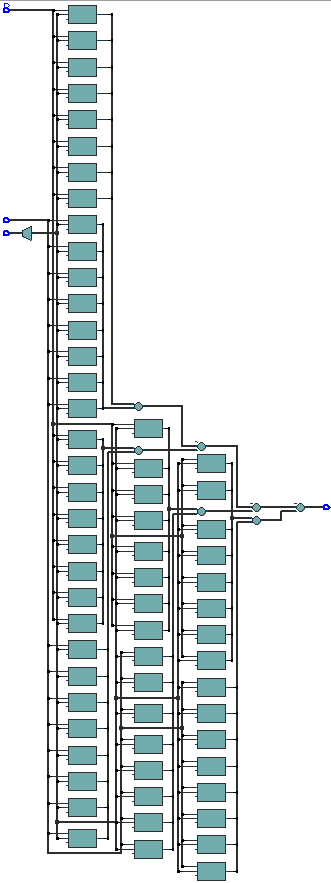
\includegraphics[scale=0.9]{For_Loop_Verilog_RTL.png}
	\caption{Diagrama RTL del producto punto de dos vectores implementado en Verilog. \label{fig:for_loop_verilog_rtl}}
\end{figure}

\begin{figure}[ht]
	\centering
	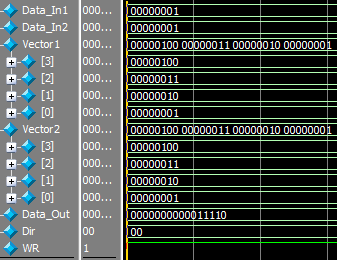
\includegraphics[scale=1.4]{For_Loop_Verilog_WaveBi.png}
	\caption{Simulación del producto punto de dos vectores en Verilog con el visor de formas de onda de ModelSim (base binaria). \label{fig:for_loop_verilog_wavebi}}
\end{figure}

\begin{figure}[ht]
	\centering
	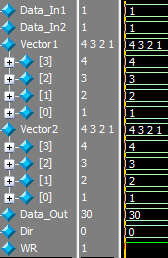
\includegraphics[scale=1.4]{For_Loop_Verilog_WaveDe.png}
	\caption{Simulación del producto punto de dos vectores en Verilog con el visor de formas de onda de ModelSim (base decimal). \label{fig:for_loop_verilog_wavede}}
\end{figure}